\documentclass[aspectratio=169]{../latex_main/tntbeamer}  % you can pass all options of the beamer class, e.g., 'handout' or 'aspectratio=43'
\usepackage{dsfont}
\usepackage{bm}
\usepackage[english]{babel}
\usepackage[T1]{fontenc}
%\usepackage[utf8]{inputenc}
\usepackage{graphicx}
\graphicspath{ {./figures/} }
\usepackage{algorithm}
\usepackage[ruled,vlined,algo2e,linesnumbered]{algorithm2e}
\usepackage{hyperref}
\usepackage{booktabs}
\usepackage{mathtools}

\usepackage{amsmath,amssymb}

\DeclareMathOperator*{\argmax}{arg\,max}
\DeclareMathOperator*{\argmin}{arg\,min}

\usepackage{amsbsy}
\newcommand{\vect}[1]{\bm{#1}}
%\newcommand{\vect}[1]{\boldsymbol{#1}}

\usepackage{pgfplots}
\pgfplotsset{compat=1.16}
\usepackage{tikz}
\usetikzlibrary{trees} 
\usetikzlibrary{shapes.geometric}
\usetikzlibrary{positioning,shapes,shadows,arrows,calc,mindmap}
\usetikzlibrary{positioning,fadings,through}
\usetikzlibrary{decorations.pathreplacing}
\usetikzlibrary{intersections}
\pgfdeclarelayer{background}
\pgfdeclarelayer{foreground}
\pgfsetlayers{background,main,foreground}
\tikzstyle{activity}=[rectangle, draw=black, rounded corners, text centered, text width=8em]
\tikzstyle{data}=[rectangle, draw=black, text centered, text width=8em]
\tikzstyle{myarrow}=[->, thick, draw=black]

% Define the layers to draw the diagram
\pgfdeclarelayer{background}
\pgfdeclarelayer{foreground}
\pgfsetlayers{background,main,foreground}

% Requires XeLaTeX or LuaLaTeX
%\usepackage{unicode-math}

\usepackage{fontspec}
%\setsansfont{Arial}
\setsansfont{RotisSansSerifStd}[ 
Path=../latex_main/fonts/,
Extension = .otf,
UprightFont = *-Regular,  % or *-Light
BoldFont = *-ExtraBold,  % or *-Bold
ItalicFont = *-Italic
]
\setmonofont{Cascadia Mono}[
Scale=0.8
]

% scale factor adapted; mathrm font added (Benjamin Spitschan @TNT, 2021-06-01)
%\setmathfont[Scale=1.05]{Libertinus Math}
%\setmathrm[Scale=1.05]{Libertinus Math}

% other available math fonts are (not exhaustive)
% Latin Modern Math
% XITS Math
% Libertinus Math
% Asana Math
% Fira Math
% TeX Gyre Pagella Math
% TeX Gyre Bonum Math
% TeX Gyre Schola Math
% TeX Gyre Termes Math

% Literature References
\newcommand{\lit}[2]{\href{#2}{\footnotesize\color{black!60}[#1]}}

%%% Beamer Customization
%----------------------------------------------------------------------
% (Don't) Show sections in frame header. Options: 'sections', 'sections light', empty
\setbeamertemplate{headline}{empty}

% Add header logo for normal frames
\setheaderimage{
	% 
\includegraphics[height=\logoheight]{figures/TNT_darkv4.pdf}
	
\includegraphics[height=\logoheight]{../latex_main/figures/luh_logo_rgb_0_80_155.pdf}
	% 
\includegraphics[height=\logoheight]{figures/logo_tntluh.pdf}
}

% Header logo for title page
\settitleheaderimage{
	% 
\includegraphics[height=\logoheight]{figures/TNT_darkv4.pdf}
	
\includegraphics[height=\logoheight]{../latex_main/figures/luh_logo_rgb_0_80_155.pdf}
	% 
\includegraphics[height=\logoheight]{figures/logo_tntluh.pdf}
}

% Title page: tntdefault 
\setbeamertemplate{title page}[tntdefault]  % or luhstyle
% Add optional title image here
%\addtitlepageimagedefault{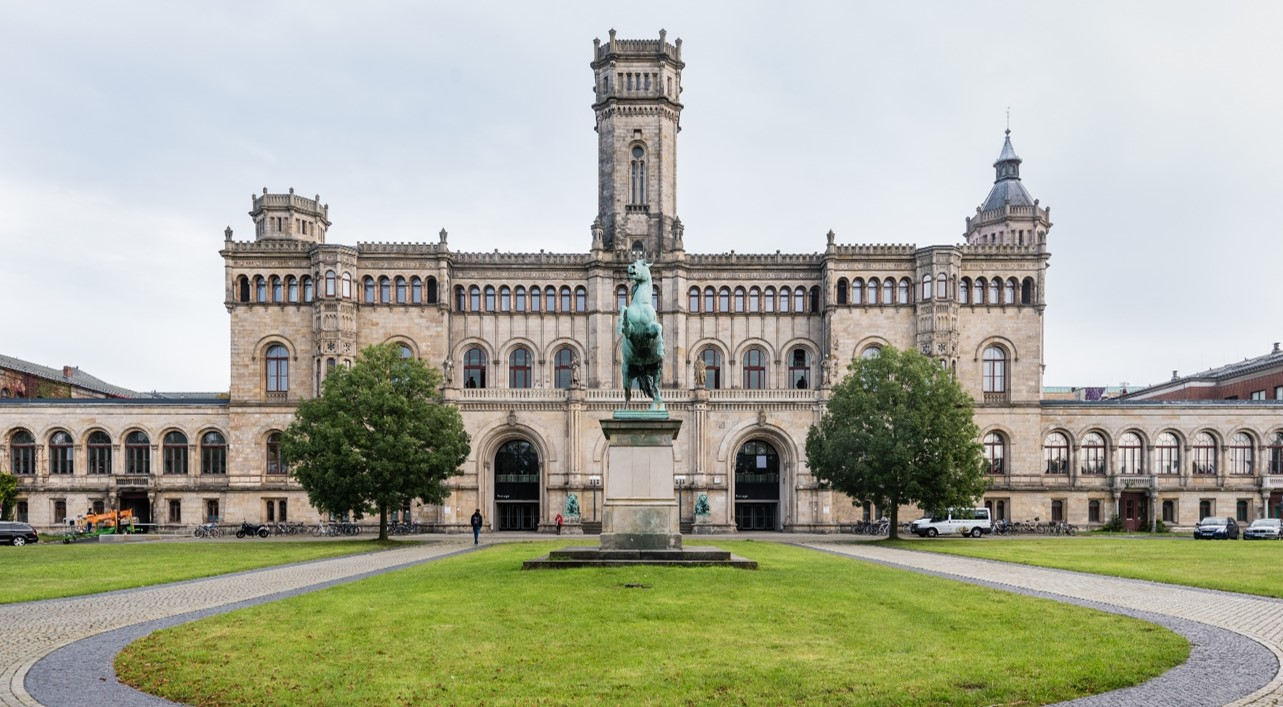
\includegraphics[width=0.65\textwidth]{figures/luh_default_presentation_title_image.jpg}}

% Title page: luhstyle
% \setbeamertemplate{title page}[luhstyle]
% % Add optional title image here
% \addtitlepageimage{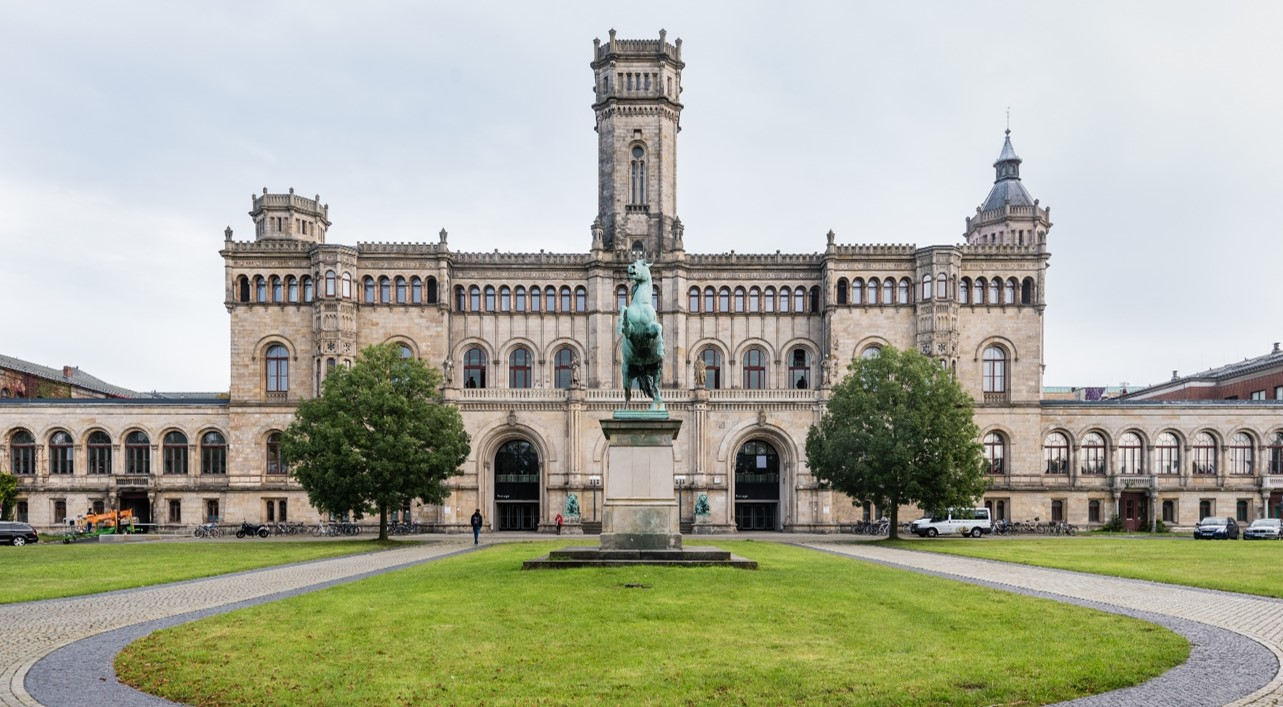
\includegraphics[width=0.75\textwidth]{figures/luh_default_presentation_title_image.jpg}}

\author[Abedjan \& Lindauer]{Ziawasch Abedjan \& Marius Lindauer\\[1em]
	
\includegraphics[height=\logoheight]{../latex_main/figures/luh_logo_rgb_0_80_155.pdf}\qquad
	
\includegraphics[height=\logoheight]{../latex_main/figures/DBIS_Kurzlogo.png}\qquad

\includegraphics[height=\logoheight]{../latex_main/figures/TNT_darkv4}\qquad

\includegraphics[height=\logoheight]{../latex_main/figures/L3S.jpg}	}
\date{Summer Term 2022; \hspace{0.5em} {
\includegraphics[height=1.5em]{../latex_main/figures/Cc-by-nc-sa_icon.svg.png}}; based on \href{https://ds100.org/fa21/}{[DS100]}
}


%%% Custom Packages
%----------------------------------------------------------------------
% Create dummy content
\usepackage{blindtext}

% Adds a frame with the current page layout. Just call \layout inside of a frame.
\usepackage{layout}


%%% Macros
%\renewcommand{\vec}[1]{\mathbf{#1}}
% \usepackage{bm}
%\let\vecb\bm

\title[Introduction]{DS: Gradient Descent}
\subtitle{Gradient Descent in 1D}

\graphicspath{ {./figure/} }
%\institute{}


\begin{document}
	
	\maketitle
	\begin{frame}{Minimizing a Function}
	    Suppose we want to minimize a function f(x) = $x^4 -15x^3 + 80x^2 - 180x +144$
	    \begin{itemize}
	        \item Many approaches for doing this.
	        \item We’ll discuss one approach today called “gradient descent”.
	    \end{itemize}
	    \centering
	    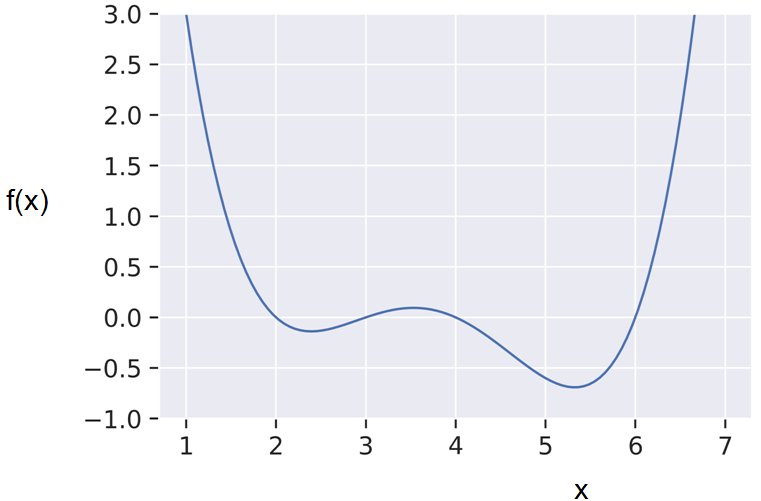
\includegraphics[scale=.38]{Bild1}
	\end{frame}
	
	
	
	\begin{frame}{Gradient Descent Intuition}
	    The intuition behind 1D gradient descent: 
	    \begin{itemize}
	        \item To the left of a minimum, derivative is negative (going down).
	        \item To the right of a minimum, derivative is positive (going up).
	        \item Derivative tells you where and how far to go.
	    \end{itemize}
	    Let’s work from here and try to invent gradient descent.\\
	    \centering
	    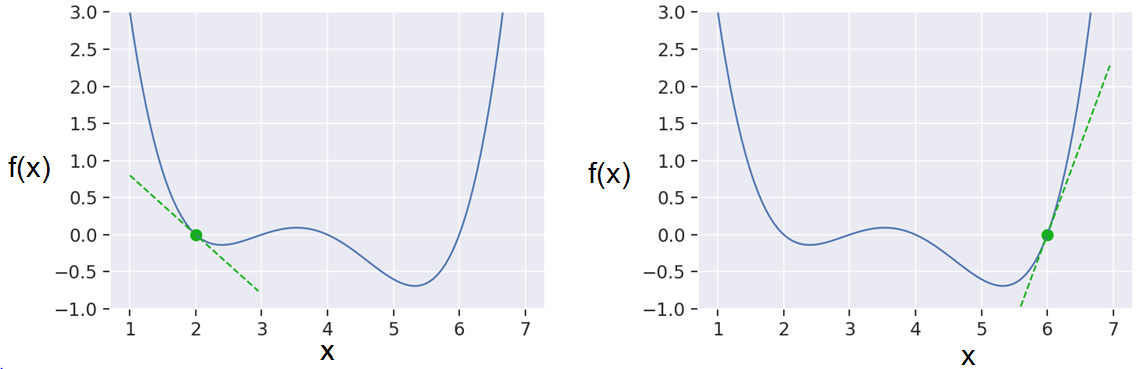
\includegraphics[scale=.38]{Bild2}
	\end{frame}
	
	
	
	\begin{frame}{Gradient Descent Algorithm}
	    The gradient descent algorithm is shown below:
	    \begin{itemize}
	        \item alpha is known as the “learning rate”.
	        \begin{itemize}
	            \item Too large and algorithm fails to converge.
	            \item Too small and it takes too long to converge.
	        \end{itemize}
	    \end{itemize}
	    \begin{equation*}
	        \hspace{-3cm}x^{(t+1)} = x^{(t)} - \alpha\frac{d}{dx}f(x)
 	    \end{equation*}
 	    
 	    
 	    \vspace{-3cm}
 	    \hspace{8.5cm} 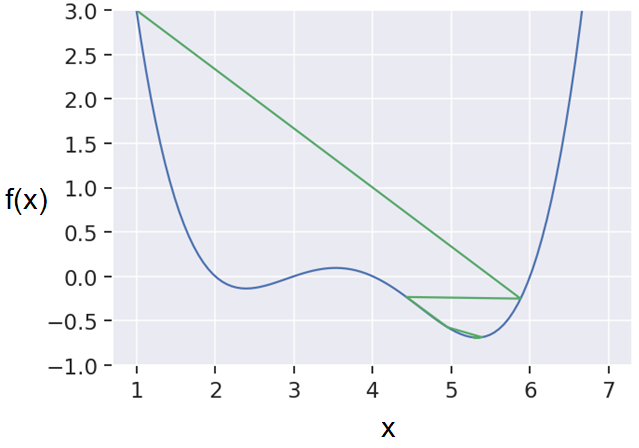
\includegraphics[scale=.35]{Bild4}\\
 	    \vspace{3cm}
 	    
 	    
 	    \vspace{-4cm}
 	    \hspace{0cm} 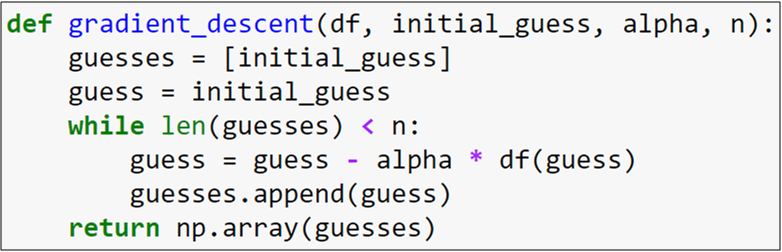
\includegraphics[scale=.5]{Bild3}\\
 	    \vspace{4cm}
	\end{frame}
	
	
	
	\begin{frame}{Gradient Descent Only Finds Local Minima}
	    \begin{itemize}
	        \item If loss function has multiple local minima, GD is not guaranteed to find global minimum.
	        \item Suppose we have this loss curve:
	    \end{itemize}
	    \centering
	    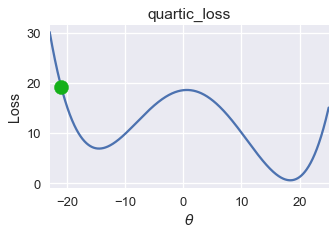
\includegraphics[scale=.7]{Bild5}
	\end{frame}
	
	
	
	\begin{frame}{Gradient Descent Only Finds Local Minima}
	    \begin{itemize}
	        \item Here’s how GD runs:
	    \end{itemize}
	    \centering
	    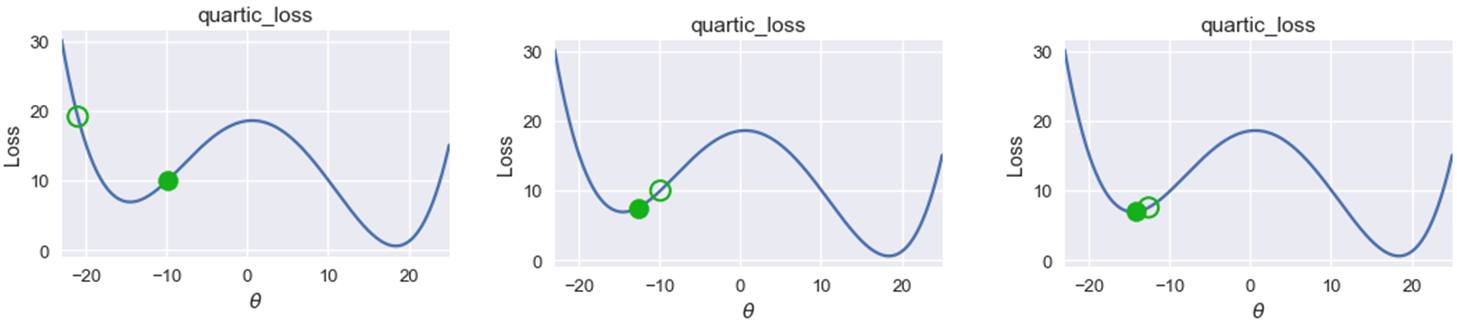
\includegraphics[scale=.4]{Bild6}
	    \begin{itemize}
	        \item GD can converge at -15 when global minimum is 18
	    \end{itemize}
	\end{frame}
	
	
	\begin{frame}{Convexity}
	    \begin{itemize}
	        \item For a convex function f, any local minimum is also a global minimum.
	        \begin{itemize}
	            \item If loss function convex, gradient descent will always find the globally optimal minimizer.
	        \end{itemize}
	        \item Formally, f is convex iff:
	    \end{itemize}
	    
	    \begin{align*}
	        tf(a)+(1-t)f(b)\geq f(ta + (1 - t)b)\\
	        \text{For all a, b in domain of f and t} \in [0,1]
	    \end{align*}
	\end{frame}
	
	
	\begin{frame}{Convexity}
	        \hspace{4cm}$tf(a)+(1-t)f(b)\geq f(ta + (1 - t)b)$\\
	        \hspace{4cm} $\text{For all a, b in domain of f and t} \in [0,1]$
	    \begin{itemize}
	        \item RTA: If I draw a line between two points on curve, all values on curve need to be on or below line.
	        \item E.g. MSE loss is convex:
	    \end{itemize}
	    \hspace{5cm}
	    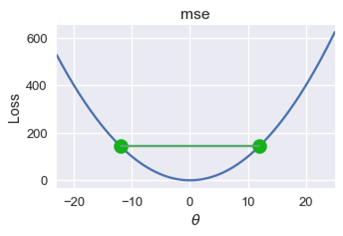
\includegraphics[scale=.4]{Bild7}
	\end{frame}
	
	
	\begin{frame}{Convexity}
	        \hspace{4cm}$tf(a)+(1-t)f(b)\geq f(ta + (1 - t)b)$\\
	        \hspace{4cm} $\text{For all a, b in domain of f and t} \in [0,1]$
	    \begin{itemize}
	        \item But this loss function is not convex:
	    \end{itemize}
	    \hspace{3.5cm}
	    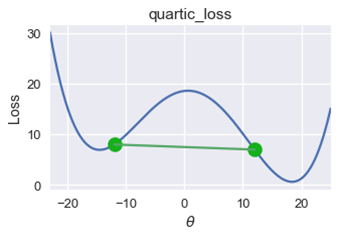
\includegraphics[scale=.5]{Bild8}
	\end{frame}
	
\end{document}